\section{Neurônios biológicos}

Neurônios são células especializadas que atuam como unidades básicas de comunicação no cérebro, transmitindo informações através
de impulsos elétricos e conexões químicas e elétricas, chamadas sinapses. Um neurônio possui três principais partes: dendritos,
soma e axônio. Dendritos recebem sinais de outros neurônios e os conduzem ao soma, onde são integrados. Se o sinal integrado
atinge um limiar, um potencial de ação, ou disparo, é gerado no axônio, propagando-se até as terminações axonais através das
sinapses, onde o sinal se propaga para os dendritos dos neurônios seguintes.

<imagem de um neurônio>

O potencial de membrana é o potencial elétrico interior da célula em relação ao exterior. Em repouso, um neurônio possui um
potencial de membrana negativo, de -40mV a -80mV, chamado potencial de repouso, que é mantido através da bomba de sódio-potássio e
da permeabilidade seletiva da membrana. Em vários neurônios, uma despolarização de aproximadamente 10mV é o suficiente para
atingir o limiar de excitação, que, uma vez atingido, desencadeia a abertura dos canais de sódio (Na+) voltagem-dependentes,
permitindo a entrada de mais Na+ e causando uma maior despolarização. Quando o potencial de membrana atinge seu pico, normalmente
por volta de +40mV, os canais de Na+ se fecham, enquanto os canais de potássio (K+) voltagem-dependentes se abrem, permitindo a
saída de K+ e repolarizando a membrana. Esse processo é seguido por uma hiperpolarização temporária, antes que o potencial de
membrana retorne ao seu estado de repouso. Essa sequência de eventos constitui um potencial de ação, que se propaga ao longo do
axônio até as sinapses, permitindo a comunicação entre os neurônios~\cite{kandelPrinciples2021}.

\begin{figure}[!ht]
\Caption{Potencial de ação, linha vermelha, condutância da membrana, envelope.}
\centering
\label{action_potential}
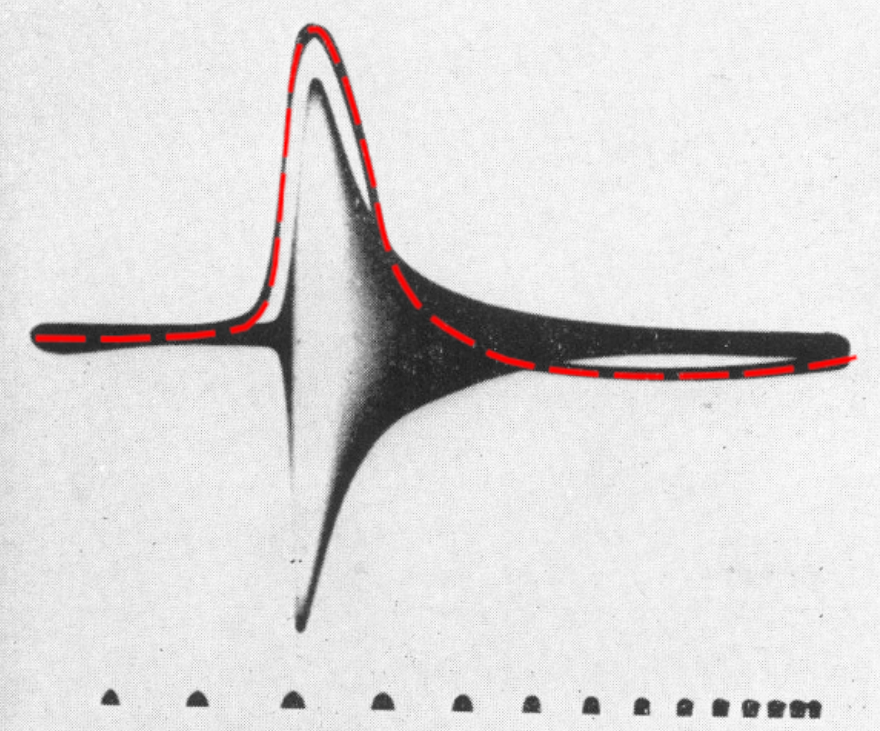
\includegraphics[width=8.5cm]{figuras/Action Potential.png}
\Fonte{Fonte.}
\end{figure}

% Imagem daqui: https://core.ac.uk/download/pdf/82621126.pdf
% Eu adicionei a linha vermelha
% Original por coleELECTRIC1939

As sinapses podem ocorrer de duas maneiras distintas: por meio de transmissão química, utilizando neurotransmissores, ou por
transmissão elétrica. Embora a transmissão química seja mais lenta, ela pode intensificar o sinal transmitido, enquanto a
transmissão elétrica é mais rápida, mas não é capaz de modificar a amplitude do sinal. As sinapses podem ter um efeito
excitatório, resultando em despolarização da célula pós-sináptica, ou um efeito inibitório, resultando em hiperpolarização. Entre
os neurotransmissores mais comuns que causam efeito excitatório estão o glutamato, a dopamina e a noradrenalina, enquanto o GABA,
a glicina e a serotonina são exemplos de neurotransmissores que exercem efeito inibitório.

Quando um potencial de ação chega à terminação axonal do neurônio pré-sináptico, vesículas contendo neurotransmissores são
liberadas na fenda sináptica. Os neurotransmissores se ligam a receptores específicos na membrana do neurônio pós-sináptico,
ativando ou inibindo os canais iônicos. Se o neurotransmissor for excitatório, ele induz a abertura de canais iônicos como os de
Na+ e Ca2+, resultando em uma entrada líquida de íons positivos e uma despolarização da membrana pós-sináptica. Por outro lado, se
o neurotransmissor for inibitório, ele geralmente causa a abertura de canais de K+ e/ou Cl-, levando à saída de íons K+ ou entrada
de íons Cl-, o que resulta em uma hiperpolarização da membrana pós-sináptica.